%----------------------------------------------------------------------------------------
%	HASIL DAN PEMBAHASAN
%----------------------------------------------------------------------------------------
\section*{HASIL DAN PEMBAHASAN}
\subsection*{Arsitektur Dokumen RDF}
Penelitian ini menggunakan dokumen tanaman obat yang didapat dari penelitian \citeauthor{HERAWAN} (\cite*{HERAWAN}). Jumlah dokumen yang digunakan berjumlah 93 dokumen dengan format XML. Dokumen dikelompokkan menjadi \textit{tag-tag} seperti pada Tabel \ref{tab:tag}.
\begin{table}[h!]
\footnotesize
\caption{Deskripsi dokumen XML tanaman obat}
\centering
\begin{tabulary}{0.45\textwidth}{LL}
\toprule
\parbox{12em}{Nama Tag} & Deskripsi \\
\midrule
$<$dok$>$&Mewakili keseluruhan dokumen\\
$<$id$>$&Menjelaskan id dokumen\\
$<$nama$>$&Nama tanaman obat\\
$<$namal$>$&Nama latin tanaman obat\\
$<$deskripsi$>$&Deskripsi tanaman obat yang terdiri dari manfaat, habitus, bagian yang digunakan dan kandungan zat kimia\\
$<$fam$>$&Famili tanaman obat\\
$<$penyakit$>$&Penyakit yang dapat disembuhkan oleh tanaman obat.\\
\bottomrule
\end{tabulary}
\label{tab:tag}
\end{table}

Dokumen XML kemudian dikonversi menjadi format dokumen RDF/XML dengan deskripsi seperti pada Tabel \ref{tab:tagRDF}. Proses konversi dilakukan secara manual sesuai dengan tag yang digunakan pada dokumen XML. Pada bagian tag $<$deskripsi$>$ terdapat manfaat, kandungan, dan lokasi yang dapat dipisahkan menjadi field yang berbeda pada dokumen RDF.
\begin{table}[h!]
\footnotesize
\caption{Deskripsi dokumen RDF tanaman obat}
\centering
\begin{tabulary}{0.47\textwidth}{LL}
\toprule
\parbox{13em}{Nama Tag} & Deskripsi \\
\midrule
$<$rdf:RDF$>$&Merupakan \textit{namespace} untuk dokumen RDF\\
$<$rdf:Description$>$&Mewakili keseluruhan dokumen\\
$<$rdf:about$>$&ID Dokumen atau  subjek pada RDF\\
$<$tanaman:famili$>$&Famili tanaman obat\\
$<$tanaman:nama$>$&Nama tanaman obat\\
$<$tanaman:latin$>$&Nama latin tanaman obat\\
$<$tanaman:habitus$>$&Habitus dari tanaman obat.\\
$<$tanaman:bagian$>$&Bagian yang digunakan pada tanaman obat\\
$<$tanaman:manfaat$>$&Manfaat dari tanaman obat\\
$<$tanaman:kandungan$>$&Kandungan dari tanaman obat\\
$<$tanaman:lokasi$>$&Lokasi tanaman obat ditemukan\\
$<$tanaman:deskripsi$>$&Deskripsi tanaman obat\\
$<$tanaman:penyakit$>$&Penyakit yang dapat disembuhkan oleh tanaman obat\\
\bottomrule
\end{tabulary}
\label{tab:tagRDF}
\end{table}

Dokumen RDF tanaman obat diberikan namespace dengan nama “tanaman”. Pada field $<$tanaman:manfaat$>$, $<$tanaman:kandungan$>$, dan $<$tanaman:lokasi$>$ dibuat dalam bentuk \textbf{rdf:Bag} karena pada beberapa dokumen tanaman obat memiliki manfaat dan kandungan yang banyak. \textbf{Rdf:Bag} merupakan tipe data dari RDF yang mendefinisikan bentuk \textit{unordered-list}.

Dokumen RDF didefinisikan menggunakan subjek, predikat, dan objek. Berikut merupakan contoh definisi pada dokumen obat Pandan Wangi:
\begin{itemize}
\item tanaman\textunderscore 1 memiliki nama Pandan Wangi.
\item tanaman\textunderscore 1 memiliki famili \textit{Pancdanaceae}.
\item tanaman\textunderscore 1 memiliki nama latin \textit{Pandanaus amaryllifolius Roxb}.
\item Bagian yang digunakan pada tanaman\textunderscore 1 adalah daun.
\item tanaman\textunderscore 1 memiliki manfaat rambut rontok, menghitamkan rambut, menghilangkan ketombe, lemah saraf, tidak nafsu makan, rematik, pegal linu, dan sakit disertai gelisah.
\item tanaman\textunderscore 1 memiliki kandungan alkaloida, saponin, flavonoida, tannin, polifenol dan zat warna
\end{itemize}

Dokumen RDF yang telah tersedia disimpan ke dalam aplikasi Sesame dengan nama repositori tanaman-obat. Kueri dibutuhkan untuk \textit{parsing} data pada dokumen RDF tanaman obat. Pada penelitian ini menggunakan bahasa kueri SPARQL.

\subsection*{\textit{Indexing}}
\textit{Indexing} dan pencarian dilakukan dengan menggunakan Lucene. Lucene merupakan sebuah mesin pencari yang digunakan dalam membangun aplikasi ini, untuk proses \textit{indexing}, \textit{searching}, dan \textit{ranking}. Pada penelitian ini digunakan beberapa \textit{class} yang terdapat pada pustaka Lucene dan dilakukan penambahan \textit{class} yang digunakan sebagai penghubung antara pengguna dan Lucene. Struktur penggunaan \textit{class} dapat dilihat pada Gambar \ref{fig:class}.

\begin{figure}[h!] % Gunakan \begin{figure*} untuk memasukkan Gambar
\centering
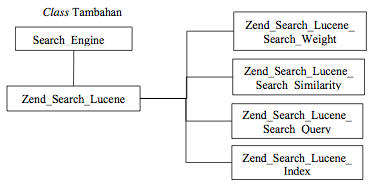
\includegraphics[width=200pt]{class.png}
\caption{Struktur penggunaan \textit{class}}
\label{fig:class}
\end{figure}

\textit{Class} \textbf{Search\textunderscore Engine} memiliki fungsi sebagai berikut:
\begin{enumerate}[noitemsep] 
\item \textbf{indexing()}, digunakan untuk melakukan fungsi indexing
\item \textbf{getManfaat()}, digunakan untuk parsing data RDF pada field manfaat dengan tipe data $<$rdf:Bag$>$
\item \textbf{getKandungan()}, digunakan untuk parsing data RDF pada field kandungan
dengan tipe data $<$rdf:Bag$>$
\item \textbf{doSearch}, digunakan untuk melakukan proses pencarian
\end{enumerate}

Pengguna memasukkan kueri yang selanjutnya akan diproses oleh fungsi \textbf{doSearch} yang terdapat pada \textit{class} \textbf{Search\textunderscore engine}. Fungsi \textbf{doSearch} dijalankan ketika terdapat kueri yang ingin dicari di dalam koleksi dokumen RDF. Fungsi \textbf{doSearch} yang selanjutnya diproses melalui \textit{search engine} Lucene. Setelah kueri diproses Lucene akan menemukembalikan dokumen yang relevan berdasarkan ranking tertinggi.

Untuk melakukan \textit{indexing}, dokumen RDF yang akan diindeks disimpan dalam sebuah aplikasi penyimpanan dokumen RDF yaitu Sesame. Proses \textit{indexing} dilakukan oleh fungsi \textbf{indexing()} yang terdapat pada \textit{class} \textbf{Search\textunderscore engine}. Fungsi \textbf{indexing()} akan melakukan \textit{parsing} data dokumen RDF pada media penyimpanan Sesame dengan menggunakan kueri SPARQL. Hasil \textit{parsing} data selanjutnya akan diindeks melalui \textit{search engine} Lucene. Hasil \textit{indexing} akan disimpan pada \textit{folder} \textbf{tmp/rdf-indeks} yang terdapat pada direktori \textbf{/xampp/htdocs/Lucene/}.

\subsection*{Pencarian}
Setelah dilakukan proses \textit{indexing}, maka dapat dilakukan pencarian pada dokumen RDF tanaman obat. Pencarian dilakukan dengan memasukkan kueri pada sistem \textit{search engine}. Jumlah kueri yang digunakan pada penelitian ini adalah 29 kueri. Kueri pada sistem ini dapat berupa kata tunggal, frase, dan gabungan dari \textit{field} yang dipilih dengan kata tunggal atau frase. Kueri akan diproses oleh sistem Lucene yang akan me-\textit{retrieve} dokumen yang relevan beserta skoringnya. Pada Lucene, jika hasil skoring lebih besar dari 1.0 maka nilai skoring akan dibulatkan menjadi 1.0. Tabel \ref{tab:hasilkueri} ditunjukkan hasil temu kembali terhadap dokumen RDF tanaman obat.

\begin{table}[h!]
\footnotesize
\caption{Hasil temu kembali dokumen RDF tanaman obat}
\centering
\begin{tabulary}{0.47\textwidth}{RLRR}
\toprule
No.&\parbox{8em}{Kueri} & \textit{Retrieved} & Relevan \\
\midrule
1. & Kanker & 3 & 3\\
2.&Flu&2&2\\
3.&Diabetes&17&17\\
4.&Pusing&3&3\\
5.&Merambat&1&1\\
6.&Menjari&2&2\\
7.&Bergerigi&15&11\\
8.&Menyirip&19&14\\
9.&Vitamin&16&15\\
10.&Antioksidan&1&1\\
11.&Protein&6&3\\
12.&Kalsium&13&8\\
13.&Diseduh&12&11\\
14.&Ditumbuk&13&12\\
15.&Diperas&7&7\\
16.&Batuk Pilek&27&3\\
17.&Kencing Batu&47&4\\
18.&Datang Bulan&13&3\\
19.&Gatal-gatal&11&4\\
20.&Sesak Nafas&9&6\\
\bottomrule
\end{tabulary}
\label{tab:hasilkueri}
\end{table}

Kueri ditentukan dengan cara memilih kata tunggal atau frase yang mewakili isi setiap tanaman obat. Kata-kata tersebut berkaitan dengan penyakit yang dapat disembuhkan, kandungan kimia, karakter fisik, dan cara penggunaan tanaman obat. Pada Lucene disediakan fitur \textit{term boosting} yang dapat meningkatkan tingkat akurasi hasil temu kembali informasi. Pada penelitian ini, tiga kueri yang memiliki tingkat akurasi yang rendah diberikan \textit{term boosting} seperti pada Tabel \ref{tab:hasilboosting}.

\begin{table}[h!]
\footnotesize
\caption{Kueri dengan \textit{term boosting}}
\centering
\begin{tabulary}{0.47\textwidth}{RLRR}
\toprule
No.&\parbox{8em}{Kueri} & \textit{Retrieved} & Relevan \\
\midrule
1. & obat diseduh(4)&42&4\\
2. & obat ditumbuk(4)&39&8\\
3. & buah diperas(4)&60&3\\ 
\bottomrule
\end{tabulary}
\label{tab:hasilboosting}
\end{table}

\subsection*{Evaluasi}
Evaluasi kinerja search engine dilakukan menggunakan nilai interpolasi maksimum \textit{recall} dan \textit{precision}. Pengujian dilakukan terhadap 29 kueri berupa kata tunggal atau frase dan dokumen yang relevan. Setiap kueri akan dihitung nilai \textit{precision} pada setiap nilai \textit{recall} standar yatu 0, 0.1, 0.2, 0.3, 0.4, 0.5, 0.6, 0.7, 0.8, 0.9, 1.0. Setelah didapatkan nilai \textit{precision} pada sebelas nilai \textit{recall} untuk setiap kueri, kemudian dicari nilai interpolasi maksimum \textit{recall} dan \textit{precision}. Nilai interpolasi maksimum \textit{recall} dan \textit{precision} dapat dilihat pada Gambar \ref{fig:recall}.
\begin{figure}[h!]\centering 
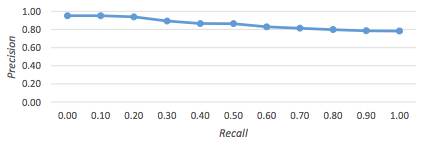
\includegraphics[width=200pt]{recall.png}
\caption{Rataan \textit{recall precision} dengan interpolasi maksimum}
\label{fig:recall}
\end{figure}

Dari percobaan yang dilakukan terhadap 29 kueri didapatkan nilai \textit{precision} sebesar 0.862. Dapat disimpulkan bahwa kinerja sistem temu kembali informasi memiliki tingkat keakuratan yang baik untuk semua kueri yang diberikan.

Dokumen yang tidak relevan tetapi tetap ditemukembalikan terjadi pada kueri ‘Batuk Pilek’, ‘Kencing Batu’, ‘Datang Bulan’, ‘Gatal-gatal’, ‘Buah Diperas’, ‘Tanaman Hias’, ‘Tumbuhan Merambat’, ‘Daun Elips’, ‘Buah Buni’, ‘Kalsium Oksalat, ‘Zat Warna’, ‘Obat Diseduh’, dan ‘Obat Ditumbuk. Hal ini disebabkan karena kueri tersebut memiliki banyak arti dalam setiap dokumen tanaman obat, sehingga tidak mampu mewakili informasi yang diinginkan pengguna. Misalnya pada kueri ‘Tumbuhan Merambat’ informasi yang diinginkan pengguna adalah mengenai tanaman obat yang tumbuh merambat, tetapi sistem akan menemukembalikan dokumen yang mengandung kata ‘Tumbuhan’ dan ‘Merambat’. Hal tersebut yang mempengaruhi nilai \textit{precision} yang didapat pada penelitian ini. Hal ini terbukti dengan menghilangkan kueri dua kata mengakibatkan perubahan nilai \textit{recall} dan \textit{precision} seperti terlihat pada Gambar \ref{fig:boosting}.
\begin{figure}[h!]\centering 
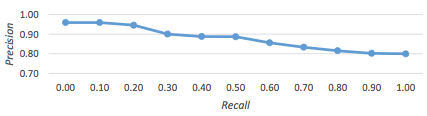
\includegraphics[width=200pt]{boosting1.png}
\caption{\textit{Recall precision} untuk kueri kata tunggal}
\label{fig:boosting}
\end{figure}

\vfill\eject % memaksa pindah kolom/halaman
Untuk kueri dengan dua kata, perlu ditambahkan penguatan pada kata tertentu dengan menggunakan \textit{term boosting} agar sistem dapat mengetahui kata yang dipentingkan. Dengan menambahkan \textit{term boosting}, nilai rataan \textit{precision} yang didapatkan lebih baik yaitu 0.877. Pada evaluasi ini juga dilakukan perhitungan \textit{recall} dan \textit{precision} dengan menggunakan nilai \textit{term boosting} yang berbeda pada masing-masing kueri yang menggunakan dua kata yaitu ‘Obat Diseduh(6)’, ‘Obat Ditumbuk(6)’, dan ‘Buah Diperas(6)’. Nilai \textit{recall} dan \textit{precision} yang dihasilkan setelah nilai \textit{term boosting} ditambahkan dapat dilihat pada Gambar \ref{fig:boosting2}.
\begin{figure}[h!]\centering 
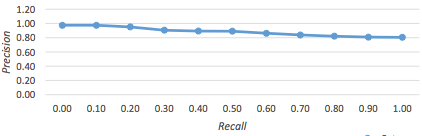
\includegraphics[width=200pt]{boosting2.png}
\caption{\textit{Recall precision} dengan \textit{term boosting}}
\label{fig:boosting2}
\end{figure}

Nilai rataan precision yang dihasilkan dengan penambahan nilai \textit{term boosting} yaitu 0.884. Dari Gambar \ref{fig:boosting2} dapat terlihat bahwa kueri dengan menambahkan \textit{term boosting} yang makin tinggi sampai pada nilai tertentu dapat meningkatkan keakuratan hasil temukembali informasi.

\subsection*{Contoh Penulisan Algoritme}
Bagian ini adalah tambahan penulisan untuk mengetahui cara menuliskan algoritme yang diacu maupun yang tidak diacu dalam teks. Algoritme \ref{algo:max} dibuat untuk mendapatkan bilangan terbesar dari kumpulan bilangan yang terhingga.
\begin{algorithm}
\DontPrintSemicolon % Some LaTeX compilers require you to use \dontprintsemicolon instead
\KwIn{Himpunan $A=\{a_1, a_2, \ldots, a_n\}$}
\KwOut{Bilangan terbesar}
$max \gets a_1$\;
\For{$i \gets 2$ \textbf{to} $n$} {
  \If{$a_i > max$} {
    $max \gets a_i$\;
  }
}
\Return{$max$}\;
\caption{{\sc Max} mendapatkan bilangan terbesar}
\label{algo:max}
\end{algorithm}

\vfill\eject % memaksa pindah kolom/halaman
\noindent Berikut adalah algoritme tanpa referensi dan caption, yang tidak diacu dalam teks:
\begin{algorithm}
\DontPrintSemicolon % Some LaTeX compilers require you to use \dontprintsemicolon instead 
\KwIn{A set $C = \{c_1, c_2, \ldots, c_r\}$ of denominations of coins, where $c_i > c_2 > \ldots > c_r$ and a positive number $n$}
\KwOut{A list of coins $d_1,d_2,\ldots,d_k$, such that $\sum_{i=1}^k d_i = n$ and $k$ is minimized}
$C \gets \emptyset$\;
\For{$i \gets 1$ \textbf{to} $r$}{
  \While{$n \geq c_i$} {
    $C \gets C \cup \{c_i\}$\;
    $n \gets n - c_i$\;
  }
}
\Return{$C$}\;
\end{algorithm}
